\documentclass[tikz]{standalone}

\usepackage{circuitikz}
\usepackage{physics}

\usetikzlibrary{calc,positioning}

\begin{document}
	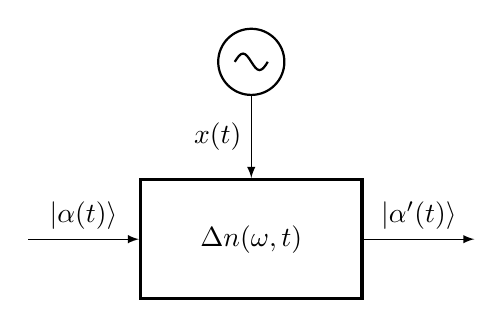
\begin{tikzpicture}[
		node distance=4em,
		arrow/.style={-latex},
		block/.style={draw, very thick, fill=white, minimum height=10ex, minimum width=8em},
	]
		\coordinate (in) at (0,0);
		\node (pc) [block, right=of in, align=center] {$\Delta n(\omega,t)$};
		node[below right] {};	
		\node (osc) [vsourcesinshape, above=3em of pc, rotate=90, anchor=west] {};
		\coordinate [right=of pc] (out);
		
		\draw[arrow] (in) -- (pc) node[above, midway] {$\ket{\alpha(t)}$};
		\draw[arrow] (pc) -- (out) node[above, midway] {$\ket{\alpha^\prime(t)}$};
		\draw[arrow] (osc.west) -- (pc.north) node[left, midway] {$x(t)$};
	\end{tikzpicture}
\end{document}
